% Überarbeitete Arbeitskopie des vom Nutzer bereitgestellten Kapitels.
% Original: trajectory_segmentation_chapter_original.tex (inhaltlich unverändert).
% Ergänzungen: deutsche Stichpunkte an den jeweiligen methodischen Stellen.
% Benchmarkabschnitte unterscheiden bestehenden Code und geplante Auswertung.
% Beide Kapiteldateien sind Alternativen und dürfen wegen gleicher Labels
% nicht gleichzeitig in dasselbe Hauptdokument eingebunden werden.
% Der aus der Vorlage übernommene Verweis tab:emission-dist wird in diesem
% Kapitelausschnitt nicht definiert und muss im Hauptdokument aufgelöst werden.

\chapter{Trajectory Segmentation and Behavioral Annotation}
\label{ch:segmentation}
The second module of our pipeline aims to identify segments within each trajectory that share similar characteristics.
These segments are assigned to \emph{states}, or recurring movement classes, where the features of segments within the same state are closer to each other than to those in other states.
Each state can optionally be assigned a biological interpretation, such as resting, foraging or traveling.
The objective is to use these groups of displacements with comparable movement properties to estimate state-dependent transition kernels.
This enables different probability distributions and step lengths depending on the distinct stages of a trajectory.

We distinguish between two types of segmentation method: data-driven and criteria-based.
Data-driven approaches learn patterns from given features and a number of states, whereas criteria-based segmentation requires user-defined rules.
The trajectories are augmented with state labels for each record and passed on to the transition-kernel module.


\section{Data-Driven Segmentation}
\label{sec:data-driven-segmentation}
Data-driven approaches, such as Hidden Markov Models (HMMs) and Behavioral Change Point Analysis (BCPA), identify patterns in a trajectory based on features like velocity and turning angle.
These features are typically calculated for each fix relative to the previous record.
Therefore, it is important that the trajectory is sampled regularly and coherently, without large gaps, so that missing records are not misinterpreted.

\subsection{Sampling-aware feature preparation}
\label{subsec:seg-preprocessing}
% Codebasis: preprocessing.py, prepare_trajectory_collection und _sampling_blocks.
Before calculating features, we identify coherent blocks of approximately constant sampling rate.
At first, each trajectory is grouped in segments according to their sampling rates within a certain tolerance band.
The dominant sampling rate $\Delta t_*$ is determined as the median of the largest interval accross all segments of the entire study.
Then, trajectories are grouped into segments with at least three fixes, where time gaps lie within a 10\% tolerance band around $\Delta t_*$:
\[
        |\Delta t_i-\Delta t_b|
        \leq a+r\Delta t_b,
        \qquad r=0.1,\quad a=1\,\mathrm{s}.
\]
Intervals outside this tolerance band interrupt a segment. 
The first two fixes of each segment serve as context for feature calculations and are not considered as model input, since displacements and turning angles require one and two preceding steps, 
respectively.
Missing observations are left missing, and steps crossing segment boundaries are not considered for the data-driven approaches. 

This way, multiple suitable segments across a study contribute to the estimation of the same motion states. 
For example, the model can learn from all segments which velocities and angles are typical.

\subsection{Features}
\label{subsec:features}
Features are attributes of a dataset from which machine learning (ML) algorithms derive patterns.
During training, ML models process the various combinations of these features and identify how they relate to the target variable.
In the case of animal trajectories, features are calculated from consecutive displacements and their time-stamps
    \[
        \mathbf{d}_i=\mathbf{x}_i-\mathbf{x}_{i-1},
        \qquad
        \Delta t_i=t_i-t_{i-1},
    \]
where $\mathbf{x}_i$ denotes the projected position at time $t_i$.
Our target variable is a number $S_i \in \{1, \ldots K\}$ denoting the behavioral state, where the user-defined variable $K$ stands for the number of expected states.


The available movement features are summarized in \Cref{tab:segmentation-features}.
For the angular features, let $\varphi_i=\operatorname{atan2}(d_{i,x},d_{i,y})$ denote the heading clockwise from north in radians, 
and let $\operatorname{wrap}$ map angular differences to $[-\pi,\pi)$.
\begin{table}[htbp]
    \centering
    \caption{Movement features available for trajectory segmentation.}
    \label{tab:segmentation-features}
    \begin{tabularx}{\textwidth}{@{}lXl@{}}
        \toprule
        Feature & Formula & Unit \\
        \midrule
        Step length
            & $\ell_i=\lVert\mathbf d_i\rVert$
            & $\mathrm{m}$ \\[0.4em]
        Speed
            & $v_i=\ell_i/\Delta t_i$
            & $\mathrm{m}/\mathrm{s}$ \\[0.4em]
        Direction
            & $h_i=(180/\pi)\varphi_i\bmod 360$
            & $ {}^\circ $ \\[0.4em]
        Signed turning angle
            & $\theta_i^{\mathrm{sgn}}=\operatorname{wrap}(\varphi_i-\varphi_{i-1})$
            & $\mathrm{rad}$ \\[0.4em]
        Turning angle
            & $\theta_i=|\theta_i^{\mathrm{sgn}}|$
            & $\mathrm{rad}$ \\[0.4em]
        Angular difference
            & $\alpha_i=(180/\pi)|\theta_i^{\mathrm{sgn}}|$
            & $ {}^\circ $ \\[0.4em]
        Persistence velocity
            & $p_i=v_i\cos\theta_i^{\mathrm{sgn}}$
            & $\mathrm{m}/\mathrm{s}$ \\[0.4em]
        Turning velocity
            & $q_i=v_i\sin\theta_i^{\mathrm{sgn}}$
            & $\mathrm{m}/\mathrm{s}$ \\[0.4em]
        Acceleration
            & $a_i=(v_i-v_{i-1})/\Delta t_i$
            & $\mathrm{m}/\mathrm{s}^2$ \\
        \bottomrule
    \end{tabularx}
\end{table}

Persistence velocity and turning velocity decompose the current velocity vector into its components along and orthogonal to the previous direction, respectively.
\begin{align}
    p_i
    &=
    \frac{1}{\Delta t_i}\mathbf d_i\cdot
    \frac{\mathbf d_{i-1}}{\lVert\mathbf d_{i-1}\rVert}
    =v_i\cos\theta_i^{\mathrm{sgn}} \in [-v_i, v_i]
    \label{eq:persistence-velocity}\\
q_i
    &=
    \frac{1}{\Delta t_i}\mathbf d_i\cdot
    \frac{\mathbf d_{i-1}^{\perp}}
         {\lVert\mathbf d_{i-1}\rVert}
    =v_i\sin\theta_i^{\mathrm{sgn}}
    \in[-v_i,v_i].
    \label{eq:turning-velocity}
\end{align}
Here, $p_i$ indicates how strong movement tends to persist from the previous direction, where positive values indicate a continuation and negative values indicate a reversal.
The turning velocity describes the lateral component to the previous velocity, where positive values correspond to turning in a clockwise direction.
Absolute directions are represented as $(\sin h_i,\cos h_i)$ pairs, so that angles around the $0^{\circ} / 360^{\circ}$ mark remain adjacent.
Redundant combinations like step length and speed, as well as more than one representation of the same turning angle or the component pair $(p_i,q_i)$ with additional speed / turning angle feature are rejected,
so the same information is not weighted multiple times.


\subsection{Hidden Markov Model}
\label{subsec:hmm}
Considering an exemplary trajectory with varying speeds and three assumed movement states, resting (R), foraging (F) and traveling (T),
we can observe time-stamped positions and derive speeds; however, the underlying states of motion are unknown.
The naive approach of assigning states from speed thresholds is impractical, as speed intervals may overlap across different states.

HMM links observable features to a hidden, temporally coherent sequence of states.

\begin{figure}[htbp]
    \centering
    \fbox{\parbox{0.9\textwidth}{
        \textbf{Grafikplatzhalter: Beispieltrajektorie}\\
        Oben: Trajektorie mit Fixes in gleichen Zeitabständen;
        geringe Punktabstände während langsamer Bewegung und
        größere Abstände während schneller Bewegung.\\
        Darunter: zugehörige Geschwindigkeit über der Zeit,
        einschließlich einiger mehrdeutiger Werte zwischen
        den beiden typischen Geschwindigkeitsbereichen.
    }}
    \caption{Illustrative trajectory and its observed movement speeds.}
    \label{fig:hmm-example}
\end{figure}


\paragraph{Hidden states and state transitions}
The hidden states $S_i \in \{R, F, T\}$ are modeled as a first-order Markov Chain, meaning that the next state, given a current state, is independent of the preceding states:
\[
        P(S_i=F\mid S_{i-1}=R,\ldots,S_1)
        =
        P(S_i=F\mid S_{i-1}=R).
\]


\begin{figure}[htbp]
    \centering
    \fbox{\parbox{0.9\textwidth}{
        \textbf{Grafikplatzhalter: Zustände und Emissionen}\\
        Links: zwei Zustandsknoten mit gerichteten
        Übergängen und Selbstschleifen entsprechend $A$.\\
        Rechts: zwei überlappende Emissionsdichten über
        der Geschwindigkeit, jeweils in derselben Farbe
        wie der zugehörige Zustand.\\
        Einen Geschwindigkeitswert im Überlappungsbereich
        markieren, der zu beiden Zuständen passen kann.
    }}
    \caption{State transitions and state-dependent emission densities.}
    \label{fig:hmm-states-emissions}
\end{figure}


Transitions probabilities between states are described via a transition matrix $A$, such that an entry $A_{RF}=0.09$ denotes the probability of transitioning from state R to state F.
\[
        A=
        \begin{pmatrix}
            0.90 & 0.09 & 0.01 \\
            0.05 & 0.90 & 0.05 \\
            0.01 & 0.09 & 0.90 \\
        \end{pmatrix}.
    \]
A start distribution is required for the first state, since there is no state preceding it.
Here,
\[
    \pi=(0.6,\;0.3,\;0.1)
\]
represents a $60\%$ probability of starting in the state R.

States are assigned distributions according to our \emph{emission} variable velocity.
The \emph{emission distribution}
\[
    V_i\mid S_i=s\sim\mathcal N(\mu_s,\sigma_s^2)
\]
describes the probability density as a normal distribution around state $S_i$, where $\mu_s$ denotes the mean speed and $\sigma_s$ stands for the standard deviation.

Using our example values from \Cref{tab:emission-dist}, a velocity of 0.4 m/s evaluates to \(
f_R(0{,}4)\approx0{,}219,
\text{ and } f_F(0{,}4)\approx0{,}444
\)
when input into the respective normal distribution densities.
This means that a velocity of 0.4 m/s fits roughly twice as well to the foraging state as to the resting state.
Given a state $S_i$, an observation is solely dependent on the emission distribution.
For $S_2 = F$, the velocity $v_2$ is evaluated using $\mathcal{N}(\mu_F=0.8, \sigma_F^2=0.25^2)$, independent of $v_1$.
However, the preceding velocities implicitly influence the current state.
As a result, observed velocities may be time-dependent overall, even though they are modeled independently for a given sequence of states.

One can evaluate a given state-sequence $s$ by multiplying the start probability alternatingly with the respective transition probabilities and emission densities.
\[
        p(s_{1:n},v_{1:n})
        =
        \pi_{s_1}f_{s_1}(v_1)
        \prod_{i=2}^{n}
        A_{s_{i-1},s_i}f_{s_i}(v_i).
\]

\begin{figure}[htbp]
    \centering
    \fbox{\parbox{0.9\textwidth}{
        \textbf{Grafikplatzhalter: HMM entlang der Zeit}\\
        Obere Zeile: verborgene Zustände $S_1,S_2,S_3$
        mit horizontalen Übergangspfeilen.\\
        Untere Zeile: beobachtete Geschwindigkeiten
        $v_1,v_2,v_3$ mit jeweils einem Pfeil vom
        zugehörigen Zustand zur Beobachtung.\\
        Übergangspfeile mit $A_{s_{i-1},s_i}$ und
        Emissionspfeile mit $f_{s_i}(v_i)$ beschriften.
    }}
    \caption{Temporal dependence structure of the hidden states and observations.}
    \label{fig:hmm-temporal-structure}
\end{figure}


For our example trajectory and a sequence $s=(R,R,R,F,T)$ this formular evaluates to:

\[
\begin{aligned}
p(s,v)
={}&
\underbrace{0{,}6}_{\text{Start in R}}
\cdot
\underbrace{4{,}9868}_{v_1=0{,}2\text{ under R}}\\
&\cdot
\underbrace{0{,}90}_{R\rightarrow R}
\cdot
\underbrace{0{,}2191}_{v_2=0{,}4\text{ under R}}\\
&\cdot
\underbrace{0{,}90}_{R\rightarrow R}
\cdot
\underbrace{4{,}9868}_{v_3=0{,}2\text{ under R}}\\
&\cdot
\underbrace{0{,}09}_{R\rightarrow F}
\cdot
\underbrace{1{,}5958}_{v_4=0{,}8\text{ under F}}\\
&\cdot
\underbrace{0{,}05}_{F\rightarrow T}
\cdot
\underbrace{0{,}9974}_{v_5=2{,}0\text{ under T}}\\
\approx{}&0{,}018965.
\end{aligned}
\]
Looking at an alternative sequence \(
s'=(R,F,R,F,T)
\), where $S_2$ with $v_2 = 0.4 m/s$ is assigned the state $F$, whose emission density is higher than for $R$, we get the transitions  \(R\rightarrow F\rightarrow R\).
Since all other factors coincide between s and s', we can evaluate s' via
\[
\frac{p(s,v)}{p(s',v)}
=
\underbrace{\frac{0{,}90\cdot0{,}90}
{0{,}09\cdot0{,}05}}_{\text{Übergänge: Faktor }180}
\cdot
\underbrace{\frac{0{,}2191}{0{,}4437}}_{\text{Emission: Faktor }0{,}494}
\approx88{,}9.
\]
As a consequence, the sequence $s$ without the alternation to the foraging state is around 89 times more likely, even though a velocity of $0.4 m/s$ generally rather indicates a foraging state.
This example underlines the strength of Hidden Markov Models compared to simple velocity thresholds, namely that HMM takes into account a combination of observations and their temporal context.

For our example trajectory with five fixes and three states, there are a total of $3^5=243$ possible sequences.
Summing over all possible sequences, we get
\[
p(v)=\sum_s p(s,v)\approx0{,}020580.
\]
Thus, the conditional probability of the best complete sequence is
\[
P(S_{1:5}=(R,R,R,F,T)\mid v)
=
\frac{0{,}018965}{0{,}020580}
\approx92{,}15\,\%.
\]

\paragraph{Viterbi and A-posteriori}
For a trajectory with $T$ movement observations and $K$ assumed states, calculating all $K^T$ possible sequence probabilities can become computationally expensive very fast.
The Viterbi algorithm is based on the idea that two subsequences ending in the same state have the same possibilities for the remaining course of the trajectory.
This is due to the Markov assumption that the next state only depends on the current state.

If one of the subsequences already has a worse evaluation, it cannot become better than the other.
Therefore, it is sufficient to keep the best partial sequence so far for each possible final state at each time step.
At the end, the best complete sequence is traced back through the stored predecessors using dynamic programming.

\begin{algorithm}[htbp]
\caption{Viterbi decoding}
\label{alg:viterbi}
\begin{algorithmic}[1]
\Require Observations $\mathbf y_{1:T}$, states $\mathcal S$,
         initial distribution $\pi$, transition matrix $A$,
         emission densities $f_s$
\Ensure Most probable state sequence $\hat s_{1:T}$

\ForAll{$s\in\mathcal S$}
    \State $\delta_1(s)\gets\pi_s f_s(\mathbf y_1)$
\EndFor

\For{$t=2,\ldots,T$}
    \ForAll{$s\in\mathcal S$}
        \State $\psi_t(s)\gets
        \operatorname*{arg\,max}_{r\in\mathcal S}
        \delta_{t-1}(r)A_{r,s}$
        \label{line:viterbi-predecessor}
        \State $\delta_t(s)\gets
        \delta_{t-1}(\psi_t(s))
        A_{\psi_t(s),s}f_s(\mathbf y_t)$
    \EndFor
\EndFor

\State $\hat s_T\gets
\operatorname*{arg\,max}_{s\in\mathcal S}\delta_T(s)$

\For{$t=T-1,\ldots,1$}
    \State $\hat s_t\gets\psi_{t+1}(\hat s_{t+1})$
    \label{line:viterbi-backtracking}
\EndFor

\State \Return $\hat s_{1:T}$
\end{algorithmic}
\end{algorithm}
The procedure detailed in \Cref{alg:viterbi} uses a $K\times T$ dimensional array $\delta$, where $\delta_t(s)$ stores the joint density of the best partial state sequence $s_{1:t}$ ending in state $s$ and the observations $\mathbf y_{1:t}$.
For the first observation, $\delta$ is initialized with the initial-state probability $\pi_s=P(S_1=s)$ multiplied with the first observation's emission density $f_s(\mathbf y_1)=p(\mathbf y_1\mid S_1=s)$.
Additionally, a $K\times T$ dimensional array $\psi$ is maintained to keep track of the best preceding state up to time $t$ for the current state ending in $s$.

For the remainder of the trajectory ($t=2,\ldots,T$), $\psi$ is updated for each state $s$ with the state maximizing
the evaluation for $t$ when transitioning from a state $r$ at $t-1$ to $s$ by multiplying the best evaluation $delta_{t-1}$ with the transition probability $A_{r,s}P(S_t=s\mid S_{t-1}=r)$ (line~\ref{line:viterbi-predecessor}).
The selected partial subsequence $\delta_t(s)$ is then extended by the current observation for each state $s$ using the best evaluation of the best predecessor of $s$ at $t - 1$ multiplied with the product
of that predecessor's transition probability to $s$ and the emission density evaluated at $\mathbf{y}_t$.
This combines the best preceding evaluation with the transition probability into
$s$ and the emission density of the current observation.
Finally, the best end state is extracted from $\delta_t(s)$, and the entire path is reconstructed backwards using the predecessor array $\psi$ (line~\ref{line:viterbi-backtracking}).

For each of the $T$ observations, $K$ possible end states with $K$ predecessors are considered, resulting in a time complexity of $\mathcal{O}(TK^2)$.

In the context of HMM, the $\textbf{A-posteriori}$ probability \(\gamma_i(s)=P(S_i=s\mid\mathbf y_{1:T})\) represents how likely the assignment of state $s$ for a step $i$ is under consideration of the entire
observation sequence.
For each step, $\gamma$ stands for a probability distribution over all states, such that \(\sum_s\gamma_i(s)=1\).
As a result, A-posteriori probabilities inform us about the ambiguity of specific state assignments.
While Viterbi outputs the most likely complete state sequence, A-posteriori describes the uncertainty of associated with individual states.
Therefore, the most likely state for a step i under A-posteriori does not necessarily coincide with Viterbi-Labels calculated using \Cref{alg:viterbi}.
We will be using A-posteriori probabilities to assign states to identified segments in our Hybrid approach detailed in \Cref{subsec:pelt-hmm-hybrid-segmentation}.

\paragraph{Multiple Features and Gaussian HMM}
In our application, we combine multiple features.
A common set of features for behavioral state annotations using animal trajectories is speed and turning angle.
In this configuration, each state has a mean vector and a covariance matrix.
\[
\boldsymbol\mu_s=
\begin{pmatrix}
\mu_{s,v}\\
\mu_{s,\theta}
\end{pmatrix},
\qquad
\Sigma_s=
\begin{pmatrix}
\sigma_{s,v}^{2} & 0\\
0 & \sigma_{s,\theta}^{2}
\end{pmatrix}.
\]
The mean values in $\mu_s$ denote typical speed values and direction changes for a state $s$.
The diagonal entries of $\sigma_s$ represent the respective variances per feature.
Entries outside the diagonal represent the covariance between different features.

We use Gaussian HMM with diagonal covariance matrices, resulting in independence of features.
Therefore, the common emission density for a step $i$, given $v_i$ and $\theta_i$ simplifies to
\[
f_s(v_i,\theta_i)
=
\mathcal N(v_i;\mu_{s,v},\sigma_{s,v}^{2})
\cdot
\mathcal N(\theta_i;\mu_{s,\theta},\sigma_{s,\theta}^{2}).
\]
For example, a state like foraging may prefer low speeds and large changes in direction.
Within this state, however, the modeled angular distribution does not additionally depend on the speed that was just observed.

\subsection{Movement Hidden Markov Model}
\label{subsec:movement-hmm}
% Codebasis: movement_hmm.py; feste Emissionsfamilie, keine freie Feature-Liste.
\begin{itemize}
    \item Zusätzlich zum Gaussian-HMM implementiert \texttt{MovementHMM} ein HMM für Schrittlänge $\ell_i$ in Metern und signierte Richtungsänderung $\theta_i^{\mathrm{sgn}}$ in Radiant. 
    Die Merkmalskombination ist fest; weitere Gaussian-Features können diesem Modell nicht beliebig hinzugefügt werden. Die Daten bleiben in physikalischen Einheiten und werden nicht standardisiert.
    \item Für positive Schrittlängen gilt zustandsabhängig $\ell_i\mid S_i=s,\ell_i>0\sim\operatorname{Gamma}(a_s,b_s)$ mit Formparameter $a_s$ und Skalenparameter $b_s$, also positivem Mittelwert $a_sb_s$. Exakte Nullschritte erhalten optional eine eigene Punktmasse $z_s$; \texttt{zero\_\allowbreak{}inflation=True} ist Standard. Ohne diese Option sind Nullschritte unzulässig und führen zu einer Fehlermeldung.
    \item Richtungsänderungen folgen einer von-Mises-Verteilung mit zustandsabhängiger, frei geschätzter mittlerer Richtung $\mu_s$ und Konzentration $\kappa_s$. Für einen beobachteten Winkel lautet die Dichte
    \[
        g_s(\theta)=\frac{\exp\!\left(\kappa_s\cos(\theta-\mu_s)\right)}{2\pi I_0(\kappa_s)},
    \]
    wobei $I_0$ die modifizierte Besselfunktion erster Art der Ordnung null bezeichnet. Kleine Konzentrationen entsprechen breiter Streuung; die Verteilung berücksichtigt die Zirkularität des Winkels.
    \item Bedingt auf den Zustand werden Schrittlänge und Drehwinkel unabhängig modelliert. Die Schrittemission ist eine gemischte Verteilung aus $P(\ell_i=0\mid S_i=s)=z_s$ und $(1-z_s)$ mal der Gamma-Dichte auf positiven Längen; bei vorhandenen Winkeln wird sie mit $g_s$ multipliziert.
    \item Besonderheit fehlender Winkel: Die gemeinsame Vorbereitung verlangt hier nur eine endliche Schrittlänge. Ein undefinierter Winkel, etwa am ersten Schritt eines Blocks, nach einem Nullschritt oder bei einer unterschwelligen Richtung, wird über eine Beobachtungsmaske ausmarginalisiert. Sein Emissionsfaktor ist eins; die bekannte Schrittlänge bleibt für Fit und Dekodierung erhalten. Ein interner numerischer Platzhalter bedeutet keine beobachtete Geradeausbewegung. Der erste Fix ohne eingehenden Schritt bleibt unmodelliert.
    \item Eigener Emissionsschätzer auf Basis von \texttt{hmmlearn.BaseHMM}: Baum--Welch mit posteriorgewichteten Gamma- und zirkulären Statistiken; numerische Nullstellensuche für Gamma-Form und von-Mises-Konzentration. Logarithmische Berechnungen und skalierte Besselfunktionen stabilisieren die Likelihood. Numerische Grenzen: $a_s\in[10^{-3},10^4]$, $b_s\geq10^{-12}$ und $\kappa_s\in[0,10^3]$.
    \item Initialisierung mit gleichverteilten Startzuständen und $A^{(0)}=0.9I+(0.1/K)\mathbf{1}\mathbf{1}^{\mathsf T}$; Emissionen aus nach Schrittlänge geschichteten, seedabhängig gestörten Gruppen. Mehrere Starts und Auswahl nach höchster endlicher Trainings-Likelihood wie beim Gaussian-HMM; Start- und Übergangswahrscheinlichkeiten werden anschließend mitgeschätzt. Eine stationäre Startverteilung wird nicht erzwungen.
    \item Abtastratengruppen, Sequenzgrenzen, Zustandsausgabe, Posterioren und Fitdiagnostik folgen der gemeinsamen HMM-Schnittstelle. Die neutrale Zustandsordnung verwendet hier die Schrittlänge. Das Modell kann wegen erhaltener Schritte mit fehlenden Winkeln eine andere Abdeckung als ein Gaussian-HMM mit derselben nominellen Merkmalskombination besitzen.
\end{itemize}

\subsection{PELT-Based Segmentation and Segment Clustering}
\label{subsec:pelt}
Our second data-driven segmentation approach is inspired by Behavioral Change Point Analysis (BCPA) and aims to identify
multiple change points, where the statistical properties of the selected feature differ significantly.
At first, temporal boundaries are identified, resulting in a set of segments, where the properties within a segment are homogonous but differ between segments.
Subsequently, these segments are grouped, given a user-input number of states, such that segments displaying similar characteristics
are assigned the same state.

\paragraph{Penalized Segmentation}
The PELT (Pruned Exact Linear Time) algorithm uses dynamic programming to find the optimal segmentation of a time-series.
Given, a series of observations $\mathbf{y}_{1:T}$, PELT identifies changepoints $0=\tau_0<\tau_1<\cdots<\tau_m=T$, where segment
$j$ contains the observations $\mathbf y_{\tau_{j-1}+1:\tau_j}$.

The algorithm minimizes a total cost
 \[
       \textsc{TotalCost} = \min_{\tau_1,\ldots,\tau_{m-1}}
        \left[
            \sum_{j=1}^{m}
            C\!\left(
                \mathbf y_{\tau_{j-1}+1:\tau_j}
            \right)
            +\beta(m-1)
        \right].
    \]
consisting of the sum of the costs for each segment ($C$) and a penalty ($\beta$) for each change point introduced.
Thus, introducing a new change point pays off if the reduction in segment costs outweighs the additional penalty.
Larger $\beta$ values encourage fewer, longer segments, where the algorithm requires larger changes in the data to justify adding boundaries.
A low penalty favors a fine partition, where subtle changes can create new segments, however at the risk of overfitting and misinterpreting noise as change points.
Additionally, a minimum allowable number of prepared movement observations per segment can be configured to discourage very short segments.

\paragraph{RBF segment cost}
Depending on the application, several segment cost functions $C_{a:b}$ can be considered.
A simple example is the L2-cost function
\[
    C(\mathbf y_{a:b}) = \sum_{i=a}^{b}\lVert\mathbf y_i-\overline{\mathbf y}_{a:b}\rVert^2.
\]
measuring the within segment sum of square deviations from the segment mean.
Given that deviations from the mean are squared, the L2 function is highly sensitive to changes in the mean and outliers and therefore performs best in applications,
where observations withing a segment are normally distributed around the mean.

A more suitable similarity measure for our application is the Radial-Basis-Function-Kernel\[
        k(\mathbf y_i,\mathbf y_j)
        =
        \exp\!\left(
            -\gamma
            \lVert\mathbf y_i-\mathbf y_j\rVert^2
        \right).
    \].
Similar feature vectors are assigned a score near one, while dissimilar ones evaluate to zero.
The parameter $\gamma$ defines the scale on which feature differences become relevant and is determined via the following median heuristic.
At first, the squared pair-wise distances of all the different observations are calculated:
\[
d_{ij}^{2}=\lVert\mathbf y_i-\mathbf y_j\rVert^2,
\qquad i<j.
\]

Then, the median is calculated from these values and $\gamma$ is set to $\gamma = 1 / M$.
Consequently, a pair with a squared distance of $M$ results in a similarity of \(
k=\exp(-\gamma M)=\exp(-1)\approx0{,}368.
\), meaning the comparison scale automatically adjusts to the observed differences in characteristics.
A common $\gamma$ value is determined for each prepared sequence so that candidate segment costs within that sequence are compared on the same scale.

The segment costs are described as variance in the feature space induced by the kernel $\textbf{k}$ as:
\[
        C(I)
        =
        \sum_{i\in I}k(\mathbf y_i,\mathbf y_i)
        -
        \frac{1}{|I|}
        \sum_{i,j\in I}k(\mathbf y_i,\mathbf y_j).
    \]
The first term simplifies to $n$, as every observation has a self-similarity of one.
Thus, $C(I)$ can be re-written as
\[
C(I)=n\left(1-\overline{k}_I\right),
\qquad
\overline{k}_I=
\frac1{n^2}\sum_{i,j\in I}k(\mathbf y_i,\mathbf y_j).
\]
Here, $\overline{k}_I$ describes the average pair-wise similarity.
If all observations are identical, $\overline{k}_I=1$ and therefore $C(I)=0$.
With varying observations, the average similarity sinks and the costs increase.
Multiplying with $n$ turns average similarity within a segment to a global segment cost.

\paragraph{Grouping segments into movement states}
The detected segments are grouped into recurring movement states.
Feature means, standard deviations and medians form segment descriptors $\mathbf{z_j}$
Given a desired number of states $K$, segments are grouped using $K$-means clustering on the standardized descriptors.
$K$-means represents every cluster through a centroid and minimizes the sum of squared distances of segment descriptors to their assigned centroids.

\subsection{PELT-HMM Hybrid segmentation}
\label{subsec:pelt-hmm-hybrid-segmentation}
The hybrid uses the PELT algorithm to identify temporal boundaries and Gaussian HMM to identify the state of each segment.
The HMM is fitted on the full prepared feature sequence, using the same fitting process as the standalone HMM.
There are two modes for state identification:
The first one uses A-posteriori probabilities, such that the state $\hat{s}_j$ maximizing the within segment sum of A-posteriori probabilities is assigned
to that segment
\[
\hat s_j=\arg\max_s\sum_{i\in I_j}
P(S_i=s\mid Y_{1:n},\hat\theta).
\]
The posterior probability $P(S_i=s\mid Y_{1:n},\hat\theta)$
describes the probability of the hidden state at observation
$i$ being $s$, given the entire observation sequence.
Its sum over a segment therefore measures the expected
number of observations belonging to state $s$ within that segment.
Thus, choosing the largest sum selects the constant segment label with the greatest expected number of matching point states under those marginal probabilities.

Alternatively, states can be assigned using a majority vote over the Viterbi labels within each segment:
\[
    \hat s_j
    =
    \operatorname*{arg\,max}_s
    \sum_{i\in I_j}
    \mathbf{1}\!\left\{\hat s_i^{\mathrm{Vit}}=s\right\},
\]
where $\hat s_i^{\mathrm{Vit}}$ denotes the state at
observation $i$ in the Viterbi-decoded sequence, and
$\mathbf{1}\{\cdot\}$ equals one if its condition holds
and zero otherwise.


\section{Criteria-Based Segmentation}
\label{sec:crit-segmentation}
In criteria-based segmentation, movement phases in a trajectory are defined based on explicit spatial, temporal, or movement-related criteria.
The user defines characteristics such as limited spatial extent for resting, or low variation in movement direction for traveling.
Regarding a trajectory $\tau$ with time-stamped positions $(x_i, y_i, t_i)\, i \in \{1,  \ldots, n\}$ and a criterion $C$,
a subtrajectory $\tau[i, j]$ is \emph{valid} under $C$, if $C(i,j)$ evaluates to true.

Criteria need to be defined per desired state.
The objective is to find the minimum number of segments $\tau[s_0, s_1], \ldots, \tau[s_{k-1}, s_k]$ with $0 = s_0 < \cdots < s_k = n$
satisfying the aforementioned criteria.

\paragraph{Criteria and monotonicity}
A criterion is called \emph{decreasing monotone} if, whenever it holds on a segment, it also holds on
every subsegment.
The decreasing monotone criteria considered in this work are summarized in \Cref{tab:decreasing-criteria}.
% Requires booktabs and tabularx.

\begin{table}[htbp]
    \centering
    \caption{Decreasing monotone segmentation criteria.
    Attribute values refer to the candidate segment
    $\tau[i,j]$.}
    \label{tab:decreasing-criteria}
    \begin{tabularx}{\textwidth}{@{}lX@{}}
        \toprule
        Criterion & Validity condition \\
        \midrule

        Maximum hops &
        The number of steps satisfies $j-i\leq h_{\max}$.
        \\[0.5em]

        Speed range &
        The difference between the largest and smallest
        speed satisfies $\max(v)-\min(v)\leq\alpha_v$.
        \\[0.5em]

        Angular range of heading &
        All headings can be covered by a circular arc
        of width at most $\alpha_h$.
        \\[0.5em]

        Angular range of turning angle &
        All turning angles can be covered by a circular
        arc of width at most $\alpha_\theta$.
        \\[0.5em]

        Disk &
        All recorded positions can be covered by a disk
        of radius $r$.
        \\

        \bottomrule
    \end{tabularx}
\end{table}
The range criteria can additionally allow up to a user-defined number $q$ of outliers.
Under this condition, they remain decreasing monotone, as shrinking a segment cannot increase the number of outliers.

The disjunction and conjunction of monotone decreasing criteria is also monotone decreasing.
For exclusively decreasing monotone criteria, a Greedy strategy yields the optimal segmentation as follows:

Starting with the first two fixes, a segment $\tau[i, j]$ is extended as long as the criterion $C$ holds.
When the first extension to a fix $j'$ violates $C$, the last valid segment $\tau[i,j'-1]$ is reported.
The process is repeated from that segment's endpoint for the remainder $\tau[j'-1,n]$ until the end is reached.
The end result is a set of segments, each satisfying $C$.

On the other hand, a criterion is called \emph{increasing monotone}, if, whenever it holds on a segment, it also holds on every segment containing it.
The increasing monotone criteria considered in this work are summarized in \Cref{tab:increasing-criteria}:

\begin{table}[htbp]
    \centering
    \caption{Increasing monotone segmentation criteria.}
    \label{tab:increasing-criteria}
    \begin{tabularx}{\textwidth}{@{}lX@{}}
        \toprule
        Criterion & Validity condition \\
        \midrule

        Minimum hops &
        The number of steps satisfies $j-i\geq h_{\min}$.
        \\[0.5em]
        Minimum duration &
        The elapsed time satisfies
        $t_j-t_i>\Delta t_{\min}$.
        \\

        \bottomrule
    \end{tabularx}
\end{table}
Like with decreasing monotone criteria, the conjunction and disjunction of increasing monote criteria is also increasing monotone.
Generally, a combination of increasing and decreasing criteria like staying within a spatial range for >24h is neither increasing nor decreasing monotone.
Their are called \emph{stable} criteria, because the number of validity changes for segment starting at varying start indices $i < j$ for a fixed end index $j$, 
summed over all end indices $j = 1 \ldots n$ is in the order of $O(n)$.
Looking at the minimum duration criterion, it becomes evident that the Greedy strategy fails for such criteria, 
as extending a segment as long as the condition is satisfied, may result in a remainder that is too short to satisfy the condition.


\begin{figure}
    \centering
    \label{free-space}
    \IfFileExists{figures/chapter04/start-stop-placeholder.png}{%
        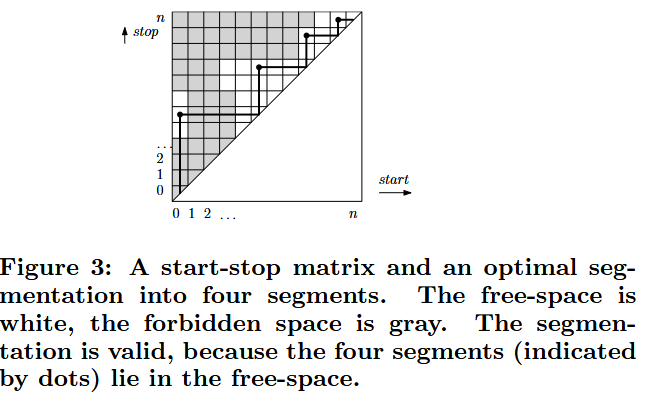
\includegraphics[width=\textwidth]{figures/chapter04/start-stop-placeholder.png}%
    }{%
        \placeholder{Start--stop diagram: add figures/chapter04/start-stop-placeholder.png.}%
    }
\end{figure}

In these cases, an optimal segmentation can be determined using a start-stop diagram $D$, where the horizontal coordinate represents the start index $i$
and the vertical coordinate denotes the end index $j$ of a candidate segment.
An entry $D(i, j)$ belongs to the \emph{free space} if its corresponding segment $\tau[i, j]$ satisfies the criterion, otherwise \emph{forbidden space}.
A segmentation of a trajectory of size $n$ corresponds to a staircase in the start-stop diagram, originating in cell $(0, 0)$ and ending in $(n, n)$.
The objective is, to find a \emph{min-link staircase} whose non-diagonal entries lie in the free space.

In their 2014 paper, Buchin et al. presented a framework that uses run-length encoding on the start-stop matrix and range queries using augmented binary-
search trees to compute the optimal segmentation for \emph{stable criteria} efficiently in $O(n\log n)$ time.

\paragraph{Combining criteria and movement states}
We define behavioral states through single criteria or the combination of multiple criteria.
For example, a set of criteria for the states resting, foraging and traveling can be defined as 
\[
\begin{aligned}
C_R &=
C_{\mathrm{disk}}(25\,\mathrm m)
\land C_{\mathrm{duration}}(300\,\mathrm s),\\
C_F &=
C_{\mathrm{disk}}(100\,\mathrm m)
\land \neg C_{\mathrm{disk}}(25\,\mathrm m),\\
C_T &=
C_{\mathrm{heading}}(35^\circ)
\land \neg C_{\mathrm{disk}}(100\,\mathrm m).
\end{aligned}
\]

Here, the resting state is characterized as a prolonged stay of at least 300 s within a confined area of radius 25 m.
The foraging state corresponds to movement within a radius of 100 m that extends beyond the resting area. 
The traveling state is described as movement in similar directions that does not remain within the foraging range.

Negations pertain to the entire candidate segment, making the criteria $C_R$, $C_F$ and $C_T$ mutually exclusive.
The three conditions are summarized to $C = C_R \vee C_F \vee C_T$, such that every segment satisfies at least one of the conditions.
A segment satisfying $C$ is then assigned the corresponding state whose condition holds on it.
\section{Implementation and Benchmark Design}
\label{sec:seg-benchmark}
The methods presented in this chapter were implemented in Python. 
Criteria-based segmentation is integrated as a wrapper on the C++ segmentation framework provided by \cite{alewijnse2014segmentation}.
The methods require \texttt{movingpandas.TrejectoryCollection} objects with metric coordinates (e.g. UTM) and return pointwise state labels together with segment boundaries.
\Cref{alg:trajectory-segmentation} summarizes their application to the prepared trajectories.

\begin{algorithm}[htbp]
\caption{Trajectory segmentation and state annotation}
\label{alg:trajectory-segmentation}
\begin{algorithmic}[1]
\Require trajectory collection $T$, method $m$, configuration $c$
\Ensure state-annotated trajectory collection $T'$
\State $T'\gets$ copy of $T$
\If{$m$ is data-driven}
    \State $B\gets$ prepared observation sequences from $T'$ \Comment{described in \Cref{subsec:seg-preprocessing}}
    \State $Y\gets$ configured movement features within each sequence in $B$
    \If{$m\in\{\text{Gaussian-HMM},\text{Movement-HMM}\}$}
        \State Fit the configured HMM jointly to $Y$, preserving sequence boundaries
        \State Decode point states with Viterbi; form segments from state runs
    \ElsIf{$m=\text{PELT-clustering}$}
        \State Detect PELT boundaries separately in each feature sequence
        \State Summarize segments and cluster their descriptors jointly into $K$ states
        \State Assign each segment's state to its observations
    \Else \Comment{PELT-HMM hybrid}
        \State Fit a Gaussian HMM jointly to $Y$, preserving sequence boundaries
        \State Detect PELT boundaries separately in each feature sequence
        \State Label each segment by posterior sums or a majority vote of Viterbi states
    \EndIf
\Else \Comment{Criteria-based segmentation}
    \ForAll{trajectories $t$ in $T'$}
        \State Find a minimum-segment partition satisfying the configured state criteria
        \State Assign the corresponding rule labels to its segments
    \EndFor
\EndIf
\State Append state labels and segment identifiers to $T'$
\State \Return $T'$
\end{algorithmic}
\end{algorithm}

An \texttt{AnnotationResult} contains the annotated collection and method-specific diagnostics.
Additionally, color-coded segments are output as plots for each trajectory.
In HMMs, segments are defined as runs of equal states. 
PELT and hybrid outputs maintain detection boundaries, even when adjacent segments are assigned the same state.

\subsection{Model choices}
\label{subsec:seg-model-choices}
\paragraph{State number and interpretation.}
The number of states $K$ is specified for the application rather than interpreted as a discovered biological truth.
AIC or BIC can guide comparisons of candidate state numbers on the same observations and feature representation.
However, additional states can also compensate for model misspecification rather than represent distinct behaviours.
The moveHMM authors recommend treating AIC as guidance and combining it with biological intuition and model assessment~\cite{Michelot2016moveHMM}.
Accordingly, $K$ should reflect the study question, expert knowledge and diagnostics of the fitted model.

\paragraph{Feature representation.}
The Gaussian HMM supports alternative feature combinations, whereas Movement-HMM uses the fixed pair $(\ell_i,\theta_i^{\mathrm{sgn}})$ without standardization.
For the planned PELT and hybrid comparison, each configuration uses one scalar feature, either persistence velocity $p_i$ or turning velocity $q_i=v_i\sin\theta_i^{\mathrm{sgn}}$.
Both combine speed with a component relative to the preceding direction; their usefulness is assessed experimentally rather than assumed from their definitions.
In the hybrid, the same scalar is supplied to PELT and its Gaussian HMM.
This is an experimental restriction, not a limitation of the multivariate implementation.

Redundant inputs can overweight the same movement information and are therefore excluded.
Examples are step length with speed at a fixed sampling interval, duplicate angular representations, or $(p_i,q_i)$ with additional speed or turning angle.
Standardization removes unit differences but not these dependencies: duplicates affect both diagonal Gaussian emission likelihoods and the distances used by PELT and clustering.

\paragraph{Shared assumptions.}
A single fit pools the retained sequences, assuming common state parameters but separate state chains.
The HMMs use time-homogeneous, first-order transitions and conditionally independent feature emissions; state durations are consequently geometric in observation steps, not explicitly modelled durations.
Neither variant includes a separate position-error model, so location error should be small relative to the displacements being interpreted.
Gaussian features are standardized over the fitted observations; PELT standardizes each input sequence and subsequently the pooled segment descriptors.
HMM parameters are estimated by Baum--Welch; among numerical initializations, the highest finite likelihood is retained, with convergence checked separately.

\subsection{Candidate studies and movement references}
\label{subsec:seg-benchmark-design}
\Cref{tab:seg-benchmark-studies} is a provisional inventory, not a final inclusion decision.
Counts refer to the local converted files before benchmark sampling selection.
The runners currently exclude Bettong by default; it remains listed to make its optional status explicit.

\begin{table}[htbp]
\centering
\small
\caption{Candidate data collections for the segmentation benchmark. Final inclusion remains open.}
\label{tab:seg-benchmark-studies}
\begin{tabularx}{\textwidth}{@{}l r >{\raggedright\arraybackslash}X@{}}
\toprule
Collection & CSVs & Available reference and main qualification \\
\midrule
Observed oystercatchers & 1 & 11,637 annotated fixes from three birds; observed behavioural labels. \\
Vlieland oystercatchers & 1 & 8,686 fixes from 18 birds; 8,611 exact matches to acceleration-derived behaviour labels. \\
Terns & 18 & 243,338 positions across four species; observed behaviour with following-boat GPS as a movement proxy. \\
Essex cattle & 1 & 12,068 positions from three animals; only 71 have exactly matched grazing/non-grazing observations. \\
Bettongs (optional) & 1 & 26,154 positions from 25 animals; provided states without an established independent observational reference. \\
\bottomrule
\end{tabularx}
\end{table}

Reference labels are grouped before choosing $K$ and scoring: sitting, standing and body care become \emph{inactive/maintenance}, food-search labels become \emph{foraging}, and walking or flying become \emph{travel}.
These are coarse movement categories, not claims of identical kinematics.
Cattle \emph{not-grazing} remains a separate complement class because it does not imply inactivity.
Original labels and the grouping table are retained.
The eighteen tern files are subdivisions of one data collection, not eighteen independent biological replications.

\subsection{Stage 1: parameter selection}
\label{subsec:seg-parameter-selection}
The following bounded candidate sets prepare the experiments; they are not reported optima.
For each study, fix the retained observation blocks and grouped reference vocabulary before comparing configurations.
Set $K$ to the number of these reference groups for the main comparison, with expert-motivated alternatives examined separately.
This uses reference knowledge for model size, not for fitting emissions or segment boundaries.

\begin{table}[htbp]
\centering
\small
\caption{Proposed parameter search. The final candidate list is fixed before the comparison.}
\label{tab:seg-parameter-search}
\begin{tabularx}{\textwidth}{@{}l >{\raggedright\arraybackslash}X >{\raggedright\arraybackslash}X@{}}
\toprule
Method & Feature candidates & Main choices \\
\midrule
Gaussian HMM & $p_i$; $q_i$; $(v_i,\theta_i)$; $(a_i,\theta_i^{\mathrm{sgn}})$; $(\ell_i,\theta_i^{\mathrm{sgn}})$ & Standardized features; fixed $K$; the last pair is an emission-family control. \\
Movement-HMM & $(\ell_i,\theta_i^{\mathrm{sgn}})$ & Zero-step point mass enabled; disable only if all supplied steps are positive. \\
PELT-clustering & $p_i$ or $q_i$, separately & $\beta\in\{0.5,2,8\}$, $m_{\min}\in\{2,3,5\}$; $\texttt{jump}=1$. \\
PELT-HMM & $p_i$ or $q_i$, separately & Same grid, with posterior-sum and majority-vote aggregation. \\
Criteria & Spatial, temporal and directional rules & Small study-specific grids of disk radii, minimum durations and heading ranges. \\
\bottomrule
\end{tabularx}
\end{table}

The proposed grid contains 18 PELT and 36 hybrid configurations per study; any refinement is documented separately.
Minimum sizes are observation counts, so their corresponding durations must also be reported.
The common HMM fitting budget is 150 EM iterations and three initializations, rather than tuning seeds against reference scores.
Select configurations by a predeclared Macro-IoU criterion, considering coverage and fit status; distinguish a shared configuration from study-specific optima.

The editable HMM runner already accepts feature candidates, and the shared runner evaluates explicit PELT/hybrid configuration lists.
The Oystercatcher parameter-search and PELT-sweep scripts provide existing grid-search patterns.
Applying the proposed search across the selected studies and freezing the winning configurations remains an experimental step; the current example lists are not search results.
Criteria segmentation still requires an adapter to the common study runner.

\subsection{Stage 2: evaluation of fixed configurations}
\label{subsec:seg-method-comparison}
\begin{itemize}
    \item Compare the frozen configurations on the same retained blocks and eligible reference points, excluding the two context fixes per block from scoring.
    Different feature requirements may still produce different prediction coverage.
    \item Match neutral states to reference groups with a one-to-one assignment maximizing summed class IoU.
    Report Macro-IoU, Macro-F1, balanced accuracy and coverage; state-wise accuracy is $100\,\mathrm{TP}_s/(\mathrm{TP}_s+\mathrm{FN}_s)$, i.e. recall in percent.
    Missing predictions count as errors; unknown reference labels are not scored.
    \item Report detection-segment counts and final state-run counts separately, together with recorded run time and fit diagnostics.
    The current timer includes sampling selection and diagnostic/export work, so it is not a pure model-fitting time.
    \item Present per-study results and collection-level summaries, plus selected spatial and state-sequence plots.
    Do not treat the number of tern CSVs as independent replication or let that subdivision determine the overall ranking.
\end{itemize}

The current runner fits and scores on the same observations and learns the state-label correspondence from those references.
Parameter selection using these scores is therefore descriptive in-sample tuning.
A claim about generalization would require a separate development/test design with frozen preprocessing and state correspondence; that split is not currently implemented.
Numerical results and the final study selection remain to be filled in.

\subsection{Planned moveHMM reference}
\label{subsec:seg-movehmm-reference}
An R moveHMM fit is planned as an additional reference on the same steps, turns, sequence boundaries and evaluation cohort.
The existing \texttt{movehmm\_\allowbreak{}reference.R} is a starting point, not yet a common-runner adapter.
Before comparison, harmonize zero-step and missing-angle treatment, angular means and initial-state assumptions; the existing R script fixes angular means at zero and uses a stationary start distribution, whereas the Python variant estimates both freely.
No numerical equivalence is assumed before this comparison is run.

\subsection{Reproducible experiment output}
\label{subsec:seg-reproducibility}
The shared runner in \texttt{benchmarks/\allowbreak{}hmm\_\allowbreak{}studies.py} records each effective configuration and its scores, point predictions, class metrics and fit diagnostics as CSV files, alongside reference-group mappings and input/code/version metadata.
The editable entry points are \texttt{run\_\allowbreak{}hmm\_\allowbreak{}studies.py} and \texttt{run\_\allowbreak{}pelt\_\allowbreak{}hybrid\_\allowbreak{}studies.py}; saved run references can be plotted without refitting.
Configuration names are identifiers only: feature lists and aggregation settings must be read from the saved effective options.
% Redaktion: Aktuelle Beispiele verwenden acceleration + signed_turn_angle (Gaussian)
% sowie speed (PELT/Hybrid) und majority_vote trotz des Namens pelt_hmm_posterior.
% Die vorgeschlagene Suche in Tabelle tab:seg-parameter-search ist davon getrennt.
% Literatur: docs/trajectory_segmentation_references.bib zur Hauptbibliographie hinzufügen.


% Literaturhinweise; BibTeX-Schlüssel erst an die vorhandene Datenbank anpassen.
% HMM: Rabiner (1989), doi:10.1109/5.18626.
% Movement-HMM: Michelot, Langrock & Patterson (2016),
% doi:10.1111/2041-210X.12578.
% Original BCPA: Gurarie, Andrews & Laidre (2009),
% doi:10.1111/j.1461-0248.2009.01293.x.
% PELT: Killick, Fearnhead & Eckley (2012),
% doi:10.1080/01621459.2012.737745.
% Kriterienframework: Alewijnse et al. (2014),
% doi:10.1145/2666310.2666415.
% Primärdokumentation für verwendete Abhängigkeiten:
% https://hmmlearn.readthedocs.io/en/stable/tutorial.html
% https://centre-borelli.github.io/ruptures-docs/user-guide/costs/costrbf/
% https://centre-borelli.github.io/ruptures-docs/code-reference/detection/pelt-reference/
% https://cran.r-project.org/web/packages/bcpa/refman/bcpa.html
% https://scikit-learn.org/stable/modules/model_evaluation.html
% https://scikit-learn.org/stable/modules/cross_validation.html
